% -*- latex -*-
%
% The SAND document class is maintained at:
%
%    http://www.cs.sandia.gov/SANDreport
%
% This page also has instructions and documentation on commands.
%
\documentclass[12pt,report]{SANDreport}

\SANDnum{SAND20XX-XXXX}
\SANDprintDate{January 20XX}

\title{VTK-m Users' Guide \\
  \relsize{-2}Version 0.0
}
\author{Kenneth~Moreland \\
  \relsize{-2} Scalable Analysis and Visualization \\[-1ex]
  \relsize{-2} Sandia National Laboratories \\[-1ex]
  \relsize{-2} P.O. Box 5800 MS 1323 \\[-1ex]
  \relsize{-2} Albuquerque, NM 87185-1323 \\[-1ex]
  \relsize{-2} kmorel@sandia.gov
}
\SANDauthor{Kenneth~Moreland}
\date{} % Leave empty


\usepackage{amsfonts}
\usepackage{amssymb}
\usepackage{amsmath}
\usepackage{booktabs}
\usepackage{graphicx}
\usepackage{isomath}
\usepackage{varioref}
\usepackage{fancyvrb}
\usepackage{ifthen}
\usepackage{longtable}
\usepackage{cite}
\usepackage{relsize}
\usepackage{subfig}
\usepackage{xspace}

% This wonderful package allows hyphenation in tt fonts and hyphenation of
% words with underscores in them.
\usepackage[htt]{hyphenat}

% This package defines a tt font that supports boldface (albeit not very
% distinctly). The default package has no boldface for tt fonts.
\usepackage{lmodern}

\usepackage{makeidx}
\makeindex

\usepackage[pdfborder={0 0 0}]{hyperref}
\usepackage{verbatim}

\usepackage{color}
\definecolor{yellow}{rgb}{1,1,0}
\definecolor{black}{rgb}{0,0,0}
\definecolor{ltcyan}{rgb}{.75,1,1}
\definecolor{red}{rgb}{1,0,0}
\definecolor{gray}{rgb}{.6,.6,.6}
\definecolor{darkred}{rgb}{0.5,0,0}
\definecolor{darkgreen}{rgb}{0,0.5,0}

\definecolor{vtkmidentifier}{rgb}{0,0,1}
\definecolor{vtkmnamespace}{rgb}{0.5,0,0}
\definecolor{vtkmmacro}{rgb}{0.5,0,0}
\definecolor{vtkmsignature}{rgb}{0,0.5,0}

\usepackage{listings}
\lstloadlanguages{C,C++}
\lstset{fontadjust=false,basicstyle=\scriptsize\ttfamily}
%% \lstset{numbers=left, numberstyle=\tiny, stepnumber=1, numbersep=2pt}
\lstdefinelanguage{VTKm}{
  morekeywords={struct,class,public,typedef,void,template,return,operator,const,for,int},
  morekeywords={[2]Id,Id2,Id3,Scalar,Tuple,Vector2,Vector3,Vector4,
                   make_Id3,make_Vector2,make_Vector3,make_Vector4,
                   dot,NUM_COMPONENTS,
                   Extent,Extent3,Pair,
                   ExtentPointDimensions,ExtentCellDimensions,
                   ExtentNumberOfPoints,ExtentNumberOfCells,
                   ExtentPointFlatIndexToTopologyIndex,
                   ExtentCellFlatIndexToTopologyIndex,
                   ExtentPointTopologyIndexToFlatIndex,
                   ExtentCellTopologyIndexToFlatIndex,
                   WorkletMapField, WorkletMapCell,
                   WorkletGenerateTopology, WorkletInterpolatedCell,
                   WorkletGenerateKeysValues, WorkletReduceKeysValues,
                   ExecutionObjectBase,
                   TypeTraits,NumericTag,DimensionalityTag,
                   TypeTraitsRealTag,TypeTraitsIntegerTag,
                   TypeTraitsScalarTag,TypeTraitsVectorTag,
                   VectorTraits,ComponentType,HasMultipleComponents,
                   VectorTraitsTagMultipleComponents,
                   VectorTraitsTagSingleComponent,
                   Error, ErrorExecution, ErrorControl,
                   ErrorControlAssert, ErrorControlBadValue,
                   ErrorControlInternal, ErrorControlOutOfMemory,
                   DeviceAdapterTagSerial,
                   DeviceAdapterTagCuda,
                   DeviceAdapterTagOpenMP,
                   DeviceAdapterTagTBB,
                   CellAverage,
                   CellDataToPointDataGenerateKeys,CellDataToPointDataReduceKeys,
                   CellGradient,
                   Cosine,Sine,Magnitude,Square,
                   Elevation,
                   MarchingCubesClassify,MarchingCubesGenerate,
                   PointDataToCellData,
                   SliceClassify,SliceGenerate,
                   Tetrahedralize,
                   ThresholdClassify,ThresholdTopology,
                   ArrayHandle,make_ArrayHandle,
                   ArrayHandleConstant,make_ArrayHandleConstant,
                   ArrayHandleCounting,make_ArrayHandleCounting,
                   ArrayContainerControl,
                   ArrayContainerControlTagBasic,
                   ArrayContainerControlTagImplicit,
                   ArrayTransfer,
                   ArrayManagerExecution,
                   ArrayManagerExecutionShareWithControl,
                   DeviceAdapterAlgorithm, DeviceAdapterAlgorithmGeneral,
                   IteratorFromArrayPortal,
                   UniformGrid,UnstructuredGrid,
                   DispatcherMapField, DispatcherMapCell,
                   DispatcherGenerateTopology, DispatcherInterpolatedCell,
                   DispatcherGenerateKeysValues,
                   DispatcherReduceKeysValues,
                   CellField, CellVertices,
                   InterpolatedCellPoints,
                   CellTraits,NUM_VERTICES,
                   CellTagHexahedron, CellTagLine, CellTagQuadrilateral,
                   CellTagTetrahedron, CellTagTriangle, CellTagVectex,
                   CellTagVoxel, CellTagWedge,
                   CellTraits,
                   CellTopologicalDimensionsTag,
                   GridTagUniform, GridTagUnstructured,
                   NUM_VERTICES, TOPOLOGICAL_DIMENSIONS,
                   ParametricCoordinates, CellDerivative,
                   SortLess, SortGreater,
                   Max, Min,
                   Cbrt, Exp, Exp10, Exp2, ExpM1, Log, Log10, Log1P, Log2,
                   Pow, RCbrt, RSqrt, Sqrt,
                   Matrix, Matrix2x2, Matrix3x3, Matrix4x4,
                   MatrixColumn, MatrixDeterminant, MatrixIdentity,
                   MatrixInverse, MatrixMultiply, MatrixRow,
                   MatrixSetColumn, MatrixSetRow, MatrixTranspose,
                   SolveLinearSystem,
                   NewtonsMethod,
                   Ceil, Epsilon, Floor, FMod, Infinity, IsFinite, IsInf,
                   IsNan, ModF, Nan, NegativeInfinity, Remainder,
                   RemainderQuotient, Round,
                   Abs, CopySign, IsNegative, SignBit,
                   ACos, ACosH, ASin, ASinH, ATan, ATan2, ATanH, Cos, CosH,
                   Pi, Sin, SinH, Tan, TanH,
                   Cross, Magnitude, MagnitudeSquared, Lerp, Normal,
                   Normalize, RMagnitude, TriangleNormal,
                   ParametricCoordinatesToWorldCoordinates,
                   WorldCoordinatesToParametricCoordinates,
                   ParametricCoordinates,
                   TransferToOpenGL
                   },
  morekeywords={[3]VTKM_CONT_EXPORT,VTKM_EXEC_EXPORT,VTKM_EXEC_CONT_EXPORT,
                   VTKM_EXEC_CONSTANT_EXPORT,
                   VTKM_DEVICE_ADAPTER,
                   VTKM_DEVICE_ADAPTER_SERIAL,
                   VTKM_DEVICE_ADAPTER_CUDA,
                   VTKM_DEVICE_ADAPTER_OPENMP,
                   VTKM_DEVICE_ADAPTER_TBB,
                   VTKM_DEVICE_ADAPTER_ERROR,
                   VTKM_DEFAULT_DEVICE_ADAPTER_TAG,
                   VTKM_ARRAY_CONTAINER_CONTROL,
                   VTKM_ARRAY_CONTAINER_CONTROL_BASIC,
                   VTKM_ARRAY_CONTAINER_CONTROL_ERROR,
                   VTKM_DEFAULT_ARRAY_CONTAINER_CONTROL_TAG,
                   VTKM_ASSERT_CONT
                   },
  morekeywords={[4]vtkm,exec,cont,worklet,math,cuda,openmp,tbb,internal,detail},
  morekeywords={[5]ControlSignature, ExecutionSignature,
                   Field,Topology,Geometry,
                   In,Out,Point,Cell,Vertices,Values,KeyGroup,ExecObject,
                   WorkId,VisitIndex,
                   _1,_2,_3,_4,_5,_6,_7,_8,_9
                   }
}
\lstset{language=VTKm}
\lstset{
  keywordstyle=\bfseries,
  keywordstyle=[2]\color{vtkmidentifier},
  keywordstyle=[3]\color{vtkmmacro},
  keywordstyle=[4]\color{vtkmnamespace},
  keywordstyle=[5]\color{vtkmsignature}
}

\renewcommand{\lstlistlistingname}{List of Examples}
\renewcommand{\lstlistingname}{Example}

\newcommand*{\textcode}[1]{\texttt{#1}}
\newcommand*{\textnamespace}[1]{\textcode{\color{vtkmnamespace}{#1}}}
\newcommand*{\textmacro}[1]{\textcode{\color{vtkmmacro}{#1}}}
\newcommand*{\textidentifier}[1]{\textcode{\color{vtkmidentifier}{#1}}}
\newcommand*{\textsignature}[1]{\textcode{\color{vtkmsignature}{#1}}}

\newcommand*{\vtkmmacro}[1]{\textmacro{#1}\index{#1}}

\newcommand{\vtkmcontexport}{\vtkmmacro{VTKM\_CONT\_EXPORT}\index{export!control}\index{function~export}\index{method~export}\xspace}
\newcommand{\vtkmexecexport}{\vtkmmacro{VTKM\_EXEC\_EXPORT}\index{export!execution}\index{function~export}\index{method~export}\xspace}
\newcommand{\vtkmexeccontexport}{\vtkmmacro{VTKM\_EXEC\_CONT\_EXPORT}\index{export!control}\index{export!execution}\index{function~export}\index{method~export}\xspace}

\newcommand{\controlsignature}{\textsignature{ControlSignature}\index{control~signature}\index{signature!control}\xspace}
\newcommand{\executionsignature}{\textsignature{ExecutionSignature}\index{execution~signature}\index{signature!execution}\xspace}

\newcommand*{\sigtag}[1]{\textsignature{#1}\index{#1}\index{signature tags!#1}}
\newcommand*{\sigtagnum}[1]{\sigtag{\_#1}}
\newcommand*{\sigtagmod}[2]{\sigtag{#1}\textcode{(}\sigtag{#2}\textcode{)}}
\newcommand*{\sigtagmodnum}[2]{\sigtag{#1}\textcode{(}\sigtagnum{#2}\textcode{)}}

\newcommand*{\writenamespaceone}[1]{%
  \textnamespace{#1}}
\newcommand*{\writenamespacetwo}[2]{%
  \writenamespaceone{#1}\textcode{:\colonhyp}\textnamespace{#2}}
\newcommand*{\writenamespacethree}[3]{%
  \writenamespacetwo{#1}{#2}\textcode{:\colonhyp}\textnamespace{#3}}
\newcommand*{\writenamespacefour}[4]{%
  \writenamespacethree{#1}{#2}{#3}\textcode{:\colonhyp}\textnamespace{#4}}

\newcommand*{\indexnamespaceone}[1]{%
  \index{#1 namespace}\index{namespace!#1}}
\newcommand*{\indexnamespacetwo}[2]{%
  \index{#2 namespace}\index{#1::#2}\index{namespace!#1::#2}}
\newcommand*{\indexnamespacethree}[3]{%
  \index{#3 namespace}\index{#1::#2::#3}\index{namespace!#1::#2::#3}}
\newcommand*{\indexnamespacefour}[4]{%
  \index{#4 namespace}\index{#1::#2::#3::#4}\index{namespace!#1::#2::#3::#4}}

\newcommand*{\writeindexidentifierone}[2]{%
  \writenamespaceone{#1}\textcode{:\colonhyp}\textidentifier{#2}%
  \index{#2}}
\newcommand*{\writeindexidentifiertwo}[3]{%
  \writenamespacetwo{#1}{#2}\textcode{:\colonhyp}\textidentifier{#3}%
  \index{#3}}
\newcommand*{\writeindexidentifierthree}[4]{%
  \writenamespacethree{#1}{#2}{#3}\textcode{:\colonhyp}\textidentifier{#4}%
  \index{#4}}
\newcommand*{\writeindexidentifierfour}[5]{%
  \writenamespacefour{#1}{#2}{#3}{#4}\textcode{:\colonhyp}\textidentifier{#5}%
  \index{#5}}

\newcommand*{\vtkm}[1]{%
  \ifthenelse{\equal{#1}{}}%
             {\writenamespaceone{vtkm}\indexnamespaceone{vtkm}}%
             {\writeindexidentifierone{vtkm}{#1}}}
\newcommand*{\vtkmcont}[1]{%
  \ifthenelse{\equal{#1}{}}%
             {\writenamespacetwo{vtkm}{cont}\indexnamespacetwo{vtkm}{cont}}%
             {\writeindexidentifiertwo{vtkm}{cont}{#1}}}
\newcommand*{\vtkmcontinternal}[1]{%
  \ifthenelse{\equal{#1}{}}%
             {\writenamespacethree{vtkm}{cont}{internal}\indexnamespacethree{vtkm}{cont}{internal}}%
             {\writeindexidentifierthree{vtkm}{cont}{internal}{#1}}}
\newcommand*{\vtkmexec}[1]{%
  \ifthenelse{\equal{#1}{}}%
             {\writenamespacetwo{vtkm}{exec}\indexnamespacetwo{vtkm}{exec}}%
             {\writeindexidentifiertwo{vtkm}{exec}{#1}}}
\newcommand*{\vtkmexecinternal}[1]{%
  \ifthenelse{\equal{#1}{}}%
             {\writenamespacethree{vtkm}{exec}{internal}\indexnamespacethree{vtkm}{cont}{internal}}%
             {\writeindexidentifierthree{vtkm}{exec}{internal}{#1}}}
\newcommand*{\vtkmworklet}[1]{%
  \ifthenelse{\equal{#1}{}}%
             {\writenamespacetwo{vtkm}{worklet}\indexnamespacetwo{vtkm}{worklet}}%
             {\writeindexidentifiertwo{vtkm}{worklet}{#1}}}
\newcommand*{\vtkmmath}[1]{%
  \ifthenelse{\equal{#1}{}}%
             {\writenamespacetwo{vtkm}{math}\indexnamespacetwo{vtkm}{math}}%
             {\writeindexidentifiertwo{vtkm}{math}{#1}}}

\newcommand*{\vtkmcuda}[1]{%
  \ifthenelse{\equal{#1}{}}%
             {\writenamespacetwo{vtkm}{cuda}\indexnamespacetwo{vtkm}{cuda}}%
             {\writeindexidentifiertwo{vtkm}{cuda}{#1}}}
\newcommand*{\vtkmcudacont}[1]{%
  \ifthenelse{\equal{#1}{}}%
             {\writenamespacethree{vtkm}{cuda}{cont}\indexnamespacethree{vtkm}{cuda}{cont}}%
             {\writeindexidentifierthree{vtkm}{cuda}{cont}{#1}}}
\newcommand*{\vtkmopenmp}[1]{%
  \ifthenelse{\equal{#1}{}}%
             {\writenamespacetwo{vtkm}{openmp}\indexnamespacetwo{vtkm}{openmp}}%
             {\writeindexidentifiertwo{vtkm}{openmp}{#1}}}
\newcommand*{\vtkmopenmpcont}[1]{%
  \ifthenelse{\equal{#1}{}}%
             {\writenamespacethree{vtkm}{openmp}{cont}\indexnamespacethree{vtkm}{openmp}{cont}}%
             {\writeindexidentifierthree{vtkm}{openmp}{cont}{#1}}}
\newcommand*{\vtkmtbb}[1]{%
  \ifthenelse{\equal{#1}{}}%
             {\writenamespacetwo{vtkm}{tbb}\indexnamespacetwo{vtkm}{tbb}}%
             {\writeindexidentifiertwo{vtkm}{tbb}{#1}}}
\newcommand*{\vtkmtbbcont}[1]{%
  \ifthenelse{\equal{#1}{}}%
             {\writenamespacethree{vtkm}{tbb}{cont}\indexnamespacethree{vtkm}{tbb}{cont}}%
             {\writeindexidentifierthree{vtkm}{tbb}{cont}{#1}}}

\newcommand*{\vtkmopengl}[1]{%
  \ifthenelse{\equal{#1}{}}%
             {\writenamespacetwo{vtkm}{opengl}\indexnamespacetwo{vtkm}{opengl}}%
             {\writeindexidentifiertwo{vtkm}{opengl}{#1}}}

\newcommand*{\tparams}[1]{\textcode{<#1>}}

\newcommand*{\textfilename}[1]{\textsf{#1}}
\newcommand*{\vtkmheader}[2]{%
  \textfilename{#1\fshyp{}#2}\index{#1\fshyp#2}\index{#2}}

\newcommand*{\cmakevar}[1]{%
  \textsf{#1}%
  \index{#1}%
  \index{CMake configuration!#1}}

\lstnewenvironment{vtkmexample}[2][-*-]{
  \lstset{caption={#2}}
  \ifthenelse{\equal{#1}{-*-}}{}{\lstset{label=#1}}
}{
}

% Cite commands I use to abstract away the different ways to reference an
% entry in the bibliography (superscripts, numbers, dates, or author
% abbreviations).  \scite is a short cite that is used immediately after
% when the authors are mentioned.  \lcite is a full citation that is used
% anywhere.  Both should be used right next to the text being cited without
% any spacing.
\newcommand*{\lcite}[1]{~\cite{#1}}
\newcommand*{\scite}[1]{~\cite{#1}}

\newcommand{\etal}{et al.}

\newcommand*{\keyterm}[1]{\emph{#1}}

\newcommand{\fix}[1]{{\color{red}\textsc{[#1]}}}
%\newcommand{\fix}[1]{}

% Avoid putting figures on their own page.
\renewcommand{\textfraction}{0.05}
\renewcommand{\topfraction}{0.95}
\renewcommand{\bottomfraction}{0.95}

% Make sure this is big enough so that only big figures end up on their own
% page but small enough so that if a figure does have to be on its own
% page, it won't push everything to the bottom because it's not big enough
% to have its own page.
\renewcommand{\floatpagefraction}{.75}

% Environments for tightly packed lists.
\newenvironment{enumeratetight}{
  \begin{enumerate}
    \setlength{\topsep}{0pt}
    \setlength{\itemsep}{0pt}
    \setlength{\parskip}{0pt}
    \setlength{\parsep}{0pt}
    \setlength{\partopsep}{0pt}
}{
  \end{enumerate}
}

\newenvironment{itemizetight}{
  \begin{itemize}
    \setlength{\topsep}{0pt}
    \setlength{\itemsep}{0pt}
    \setlength{\parskip}{0pt}
    \setlength{\parsep}{0pt}
    \setlength{\partopsep}{0pt}
}{
  \end{itemize}
}

\newenvironment{descriptiontight}{
  \begin{description}
    \setlength{\topsep}{0pt}
    \setlength{\itemsep}{0pt}
    \setlength{\parskip}{0pt}
    \setlength{\parsep}{0pt}
    \setlength{\partopsep}{0pt}
}{
  \end{description}
}

\begin{document}

\sloppy

\maketitle

\begin{abstract}
  \fix{Write this.}
\end{abstract}

\clearpage

\chapter*{Acknowledgement}

\fix{Write this. Can steal from Dax document.}


\cleardoublepage % TOC should start on an odd page
\tableofcontents
\listoffigures
%\listoftables
\lstlistoflistings

\clearpage

\SANDmain

% -*- latex -*-

\chapter{Introduction}
\label{chap:Introduction}

High-performance computing relies on ever finer threading. Advances in
processor technology include ever greater numbers of cores, hyperthreading,
accelerators with integrated blocks of cores, and special vectorized
instructions, all of which require more software parallelism to achieve
peak performance. Traditional visualization solutions cannot support this
extreme level of concurrency. Extreme scale systems require a new
programming model and a fundamental change in how we design algorithms. To
address these issues we created VTK-m: the visualization toolkit for
multi-/many-core architectures.

VTK-m supports a number of algorithms and the ability to design further
algorithms through a top-down design with an emphasis on extreme
parallelism. VTK-m also provides support for finding and building links
across topologies, making it possible to perform operations that determine
manifold surfaces, interpolate generated values, and find adjacencies.
Although Dax provides a simplified high-level interface for programming,
its template-based code removes the overhead of abstraction.

\begin{figure}[htb]
  \centering
  \begin{tabular}{ccc}
    CUDA SDK & PISTON & VTK-m \\
    {\small 431 LOC} & {\small 369 LOC} & {\small 265 LOC} \\
    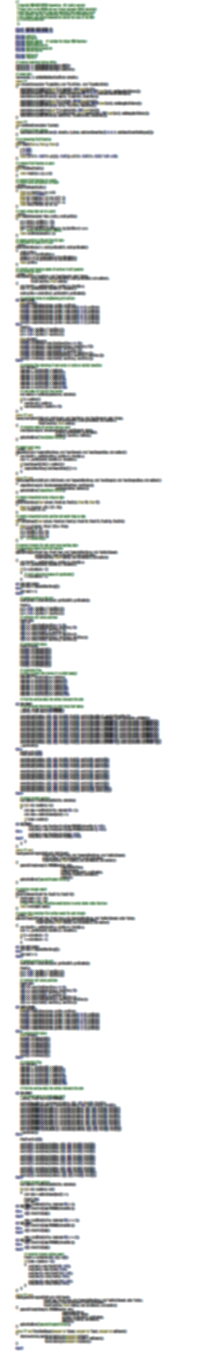
\includegraphics[width=.75in]{images/MCCompareCuda} &
    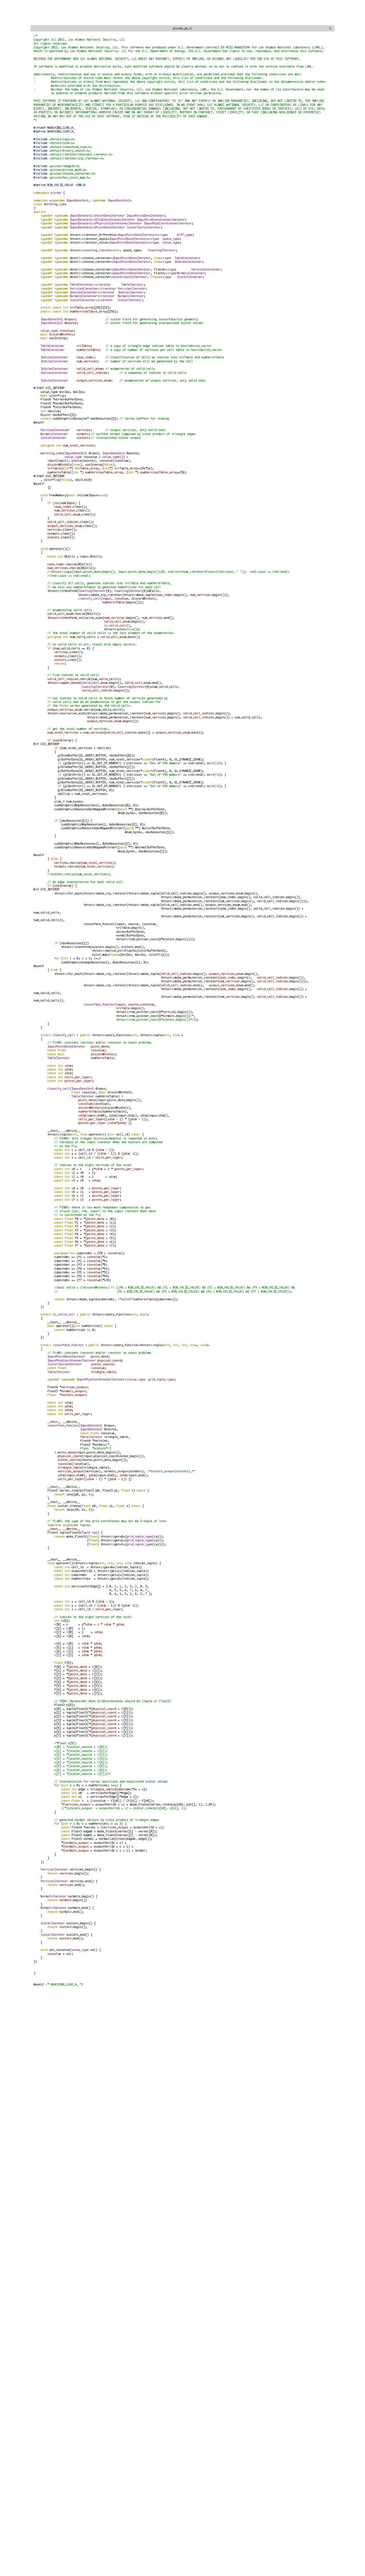
\includegraphics[width=.75in]{images/MCComparePiston} &
    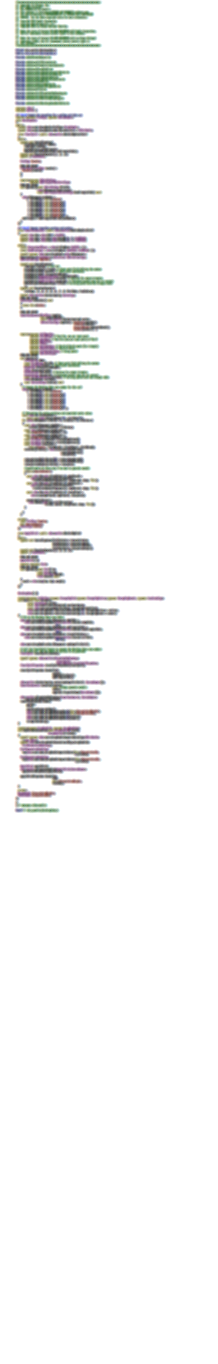
\includegraphics[width=.75in]{images/MCCompareVTKm}
  \end{tabular}
  \caption[Comparison of Marching Cubes implementations.]{Comparison of the
    Marching Cubes algorithm in VTK-m and two other implementations.
    Implementations in VTK-m are simpler, shorter, more general, and easier
    to maintain. (Lines of code (LOC) measurements come from cloc.}
  \label{fig:MCCompare}
\end{figure}

VTK-m simplifies the development of parallel scientific visualization
algorithms by providing a framework of supporting functionality that allows
developers to focus on visualization operations. Consider the listings in
Figure~\ref{fig:MCCompare} that compares the size of the implementations
for the Marching Cubes algorithm in VTK-m with the equivalent algorithms
implemented in the CUDA software development kit reference implementation
and the PISTON visualization library. Because VTK-m internally manages the
parallel distribution of work and data, the VTK-m implementation is shorter
and easier to maintain. Additionally, VTK-m provides data abstractions not
provided by the other libraries that make code written in VTK-m more
versatile.

\begin{didyouknow}
  VTK-m is written in C++ and makes extensive use of templates. The toolkit
  is implemented as a header library, meaning that all the code is
  implemented in header files (with extension \textfilename{.h}) and
  completely included in any code that uses it. This allows the compiler to
  inline and specialize code for better performance.
\end{didyouknow}

\section{How to Use This Guide}

This user's guide is organized into three parts to help guide novice to
advanced users and to provide a convenient reference.
Part~\ref{part:GettingStarted}, Getting Started, provides everything needed
to get up and running with VTK-m. In this part we learn the basics of
reading and writing data files, using filters to process data, and perform
basic rendering to view the results.

Part~\ref{part:Developing}, Developing with VTK-m, dives deeper into the
VTK-m library and provides all the information needed to customize VTK-m's
data structures and support multiple devices. Part~\ref{part:Developing}
also documents how to use VTK-m's framework to develop new or custom
visualization algorithms.

Part~\ref{part:Advanced}, Advanced Customization, exposes the inner
workings of VTK-m and allows you to design new algorithmic structures not
already available. \fix{This might be removed in the first version of the
  book.}

\section{Conventions Used in This Guide}

When documenting the VTK-m API, the following conventions are used.
\begin{itemize}
\item Filenames are printed in a \textfilename{sans serif font}.
\item C++ code is printed in a \textcode{monospace font}.
\item Macros and namespaces from VTK-m are printed in \textnamespace{red}.
\item Identifiers from VTK-m are printed in \textidentifier{blue}.
\item Signatures, described in Chapter~\ref{chap:Worklets}, and the
  tags used in them are printed in \textsignature{green}.
\end{itemize}

This guide provides actual code samples throughout its discussions to
demonstrate their use. These examples are all valid code that can be
compiled and used although it is often the case that code snippets are
provided. In such cases, the code must be placed in a larger context.

\begin{didyouknow}
  In this guide we periodically use these \textbf{Did you know?} boxes to
  provide additional information related to the topic at hand.
\end{didyouknow}

\begin{commonerrors}
  \textbf{Common Errors} blocks are used to highlight some of the common
  problems or complications you might encounter when dealing with the topic
  of discussion.
\end{commonerrors}


\chapter{Basic Provisions}
\label{chap:BasicProvisions}

\fix{Write this.}

\fix{Include package structure as section.}

\chapter{Provided Worklets}
\label{chap:ProvidedWorklets}

\fix{Write this once some worklets are provided. I expect before this we
  will have a chapter on provided filters. In fact, that probably means
  this chapter should move after the chapters on control and execution
  environments.}

\chapter{Control Environment}
\label{chap:ControlEnvironment}

\fix{Write this.}

\chapter{Execution Environment}
\label{chap:ExecutionEnvironment}

\fix{Write this.}


\begin{flushleft}
  \clearpage
  \lhead[]{}
  \rhead[]{}
  \phantomsection
  \addcontentsline{toc}{chapter}{Index}
  \printindex
\end{flushleft}

% -*- latex -*-

\begin{SANDdistribution}[NM]
  % External Addresses
  %% \SANDdistExternal{1}{Lucy Nowell\\ U.S. Department of Energy\\ SC-21\\ 19901 Germantown Road\\ Germantown, MD 20874-1290}
  %% \SANDdistExternal{1}{Teresa Beachley\\ U.S. Department of Energy\\ SC-21\\ 19901 Germantown Road\\ Germantown, MD 20874-1290}
  %% \SANDdistExternal{1}{Berk Geveci\\ Kitware, Inc.\\ 28 Corporate Drive\\ Clifton Park, NY 12065}
  %% \SANDdistExternal{1}{Robert Maynard\\ Kitware, Inc.\\ 28 Corporate Drive\\ Clifton Park, NY 12065}
  %% \SANDdistExternal{1}{Kwan-Liu Ma\\ Department of Computer Science\\ 2063 Kemper Hall\\ University of California-Davis\\ One Shields Avenue\\ Davis, CA 95616-8562}

  \bigskip

  % Internal Addresses
  \SANDdistInternal{1}{1326}{Kenneth Moreland}{1461}
  \SANDdistInternal{1}{1327}{Ron Oldfield}{01461}
\end{SANDdistribution}


\end{document}
